\documentclass[a4paper]{article}

\usepackage[polish]{babel}
	\addto{\captionspolish}{\renewcommand{\abstractname}{}}
\usepackage[OT4]{polski}
\usepackage[utf8]{inputenc}
\usepackage{amsmath}
\usepackage{graphicx}
\usepackage[colorinlistoftodos]{todonotes}
\usepackage[top = 3cm, bottom = 4cm, left = 2cm, right = 2cm]{geometry}
\usepackage{indentfirst}
\usepackage{caption}
\usepackage{subcaption}
\usepackage[nodayofweek,level]{datetime}

% Block diagram
\usepackage{mathtools}
\usepackage{amsfonts}
\usepackage{amsthm}
\usepackage{algorithm}
\usepackage[noend]{algpseudocode}
\makeatletter
	\renewcommand*{\ALG@name}{Algorytm}
\makeatother

\algnewcommand\algorithmicOutput{\textbf{Wyjście:}}
\algnewcommand\Output{\item[\algorithmicOutput]}

\algnewcommand\algorithmicInput{\textbf{Wejście:}}
\algnewcommand\Input{\item[\algorithmicInput]}

\algnewcommand\algorithmicVar{\textbf{Zmienne pomocnicze:}}
\algnewcommand\Temporary{\item[\algorithmicVar]}

\usepackage{placeins}
\usepackage{float}
\usepackage{booktabs}
\usepackage{array}
\newcolumntype{L}[1]{>{
\raggedright\let\newline\\\arraybackslash\hspace{0pt}}m{#1}}
\newcolumntype{C}[1]{>{\centering\let\newline\\\arraybackslash\hspace{0pt}}m{#1}}
\newcolumntype{R}[1]{>{\raggedleft\let\newline\\\arraybackslash\hspace{0pt}}m{#1}
}

\newcounter{rownum}	%table counter
	\newcommand\rownum{\stepcounter{rownum}\arabic{rownum}}
\setcounter{rownum}{0}

%%%%%%%%%%%%%%%%%%%%%%%%%%%%%%%%%%%%%%%%%%%%%%%%%%%%%%%%%%%%%%%%%%%%%%%%%%%%%%%%%%%%%%%%%%%%%%%%%%%
\title{Filtracja sygnałów EKG \\ Raport końcowy}

\author{Sylwia Gruszeczka, Klaudia Luks, Anna Potempa, Marta Wojciechowska, \\
Wojciech Karkoszka, Wojciech Kot, Mateusz Kozyra, Martyn Pękala}

\date{\formatdate{12}{01}{2017}}

\begin{document}
\maketitle
%%%%%%%%%%%%%%%%%%%%%%%%%%%%%%%%%%%%%%%%%%%%%%%%%%%%%%%%%%%%%%%%%%%%%%%%%%%%%%%%%%%%%%%%%%%%%%%%%%%
%%%%%%%%%%%%%%%%%%%%%%%%%%%%%%%%%%%%%%%%%%%%%%%%%%%%%%%%%%%%%%%%%%%%%%%%%%%%%%%%%%%%%%%%%%%%%%%%%%%
\section{Wstęp}

Celem raportu jest podsumowanie prac nad implementacją filtrów w środowisku MATLAB oraz w języku C++. Zrealizowane programy zostały wykorzystane do filtracji sygnałów elektrokardiograficznych, a osiągane przez nie rezultaty -- porównane ze sobą.

%%%%%%%%%%%%%%%%%%%%%%%%%%%%%%%%%%%%%%%%%%%%%%%%%%%%%%%%%%%%%%%%%%%%%%%%%%%%%%%%%%%%%%%%%%%%%%%%%%%
\section{Zaimplementowane filtry}

%%%%%%%%%%%%%%%%%%%%%%%%%%%%%%%%%% BEGINNING SG %%%%%%%%%%%%%%%%%%%%%%%%%%%%%%%%%%%%%%

\subsection{Filtr Savitzky'ego-Golaya}

\subsubsection {Wstęp}

Filtracja Savitzky'ego-Golaya polega na wygładzaniu danych wejściowych za pomocą aproksymacji wielomianu metodą najmniejszych kwadratów. Lokalne dopasowywanie wielomianów i obliczanie wartości wielomianu dla środkowego punktu analizowanego interwału jest równoważne działaniu na sygnał odpowiednim filtrem \cite{on}. Przesuwając okno, w którym następuje dopasowanie odpowiedniej krzywej, uzyskuje się -- dla środkowej próbki przedziału -- wartość wygładzoną. Filtry Savitzky'ego-Golaya mona traktować jak filtry o skończonej odpowiedzi impulsowej (FIR). Szczególnym przypadkiem tego rodzaju filtracji jest filtr ruchomej średniej (w przypadku, gdy rząd wielomianu aproksymacyjnego wynosi 0).

Co istotne, wygładzanie zaszumionego sygnału tą metodą zwiększa stosunek sygnału do szumu, ale jednocześnie dość dobrze zachowuje kształt i amplitudę poszczególnych pików. Ta własność znajduje szczególne zastosowanie w sygnałach elekardiograficznych \cite{what}, gdzie na podstawie morfologii zespołów QRS można rozpoznać wiele zaburzeń, tak więc sygnał przefiltrowany musi być jak najmniej zniekształcony. Algorytm może jednak powodować niekorzystne efekty brzegowe, które mogą zostać uniknięte poprzez nadbudowanie sygnału wejściowego na brzegach o określoną liczbę próbek.

Zalety filtracji Savitzky'ego-Golaya to tendencja do zachowywania wysokości i szerokości szczytów oryginalnego sygnału, płaska charakterystyka w zakresie pasma przepustowego i liniowe przesunięcie fazowe. Do wad algorytmu można zaliczyć pojawienie się efektów brzegowych na końcach sygnału (czemu można jednak zaradzić rozszerzając odpowiednio sygnał) oraz konieczność obliczania współczynników wielomianu dla każdorazowo przesuniętego okna, co wiąże się z kosztowną obliczeniowo operacją odwracania macierzy \cite{per-olof}.

%%%%%%%%%%%%%%%%%%%%%%%%%%%%%%%%%%%%%%%%%%%%%%%%%%%%%%%%%%%%%%%%%%%%%%%%%%%%%%%%%%%%%%%%%%%%%%%%%%%
\subsubsection {Matematyczny opis algorytmu}

Zadaniem algorytmu jest dopasowanie w kolejnych fragmentach sygnału wielomianu, który najlepiej przybliża otrzymane dane. Wyznaczanie współczynników takiego wielomianu może zostać oparte o metodę najmniejszych kwadratów \cite{least-squares} -- należy znaleźć takie, które minimalizują wartość funkcji:

\begin{equation} \label{eq1}
S(a_0, ..., a_K) = \sum_{i=1}^N \left( y_i - y(x_i) \right)^2
\end{equation}

gdzie K -- rząd dopasowywanego wielomianu, $(x_i, y_i)$ -- punkty poddawane filtracji, $y$ -- funkcja opisująca dopasowany wielomian.\\

Aby znaleźć minimum takiej funkcji możemy znaleźć miejsca, w których pochodne cząstkowe funkcji są równe zeru. Oznacza to rozwiązanie układu równań składającego się z wyrażeń dla każdej k-tej wartości współczynnika:

\begin{equation}
\frac{\delta S(a_0, ..., a_K)}{\delta a_k} = 0
\end{equation}

Zatem:

\begin{equation}
\frac{\delta}{\delta a_k} \sum_{i=1}^N \left( y_i - y(x_i) \right)^2 = 0
\end{equation}

\begin{equation}
\frac{\delta}{\delta a_k}\sum_{i=1}^N \left( y_i - \left(a _0 + ... + a_K x_i^K \right)\right)^2 = 0
\end{equation}

\begin{equation}
2\sum_{i=1}^N \left( y_i - a_0 - ... - a_K x_i^K \right) (- x_i^k) = 0
\end{equation}

Stąd otrzymać możemy układ równań o wyrazach w postaci:

\begin{equation} \label{normal_equations_for_ls}
\sum_{j=0}^K a_j \sum_{i=1}^N x_i^{j+k} = \sum_{i=1}^N y_i x_i^k
\end{equation}

Co można przedstawić w postaci macierzowej:

\begin{equation} \label{matrices}
\begin{bmatrix}
    N      & \sum_{i=1}^N x_i & \dots & \sum_{i=1}^N x_i^{K} \\
    \sum_{i=1}^N x_i      & \sum_{i=1}^N x_i^2 & \dots & \sum_{i=1}^N x_i^{K+1} \\
    \vdots & \vdots & \ddots & \vdots \\
\sum_{i=1}^N x_i^K      & \sum_{i=1}^N x_i^{1+K} & \dots & \sum_{i=1}^N x_i^{2K}\\
\end{bmatrix}
\begin{bmatrix}
    a_0	\\
    a_1	\\
    \vdots	\\
    a_N
\end{bmatrix}
=
\begin{bmatrix}
    \sum_{i=1}^N y_i	\\
    \sum_{i=1}^N y_i x_i	\\
    \vdots	\\
    \sum_{i=1}^N y_i x_i^K
\end{bmatrix}
\end{equation}

Mnożąc lewostronnie przez odwrotność pierwszej z macierzy otrzymujemy wartości współczynników:

\begin{equation}
(X^{-1}) X A = X^{-1}Y
\end{equation}

\begin{equation}
A = X^{-1}Y
\end{equation}

Kolejnym krokiem jest obliczenie wartości dopasowanego wielomianu dla jednej z próbek znajdującej się w oknie -- w omawianym przypadku jest to środek okna.

\begin{equation}
y_{filtered} = \sum_{i=1}^K a_k x_i^k
\end{equation}

\subsubsection {Opis implementacji}

Konieczność dokonywania dopasowywania wielomianu metodą najmniejszych kwadratów w określonym oknie przesuwanym po całej długości sygnału powoduje, że wykonywane operacje są złożone numerycznie. Podjęto zatem próbę znalezienia sposobu pozwalającego na optymalizację filtracji. Wykorzystując równanie normalnie dla aproksymacji metodą najmniejszych kwadratów (równanie \ref{normal_equations_for_ls}) możemy, wykonując odpowiednie przekształcenia \cite{sg-optimization-book, sg-optimization} obliczyć odpowiedź impulsową filtra dla okna o długości $2M+1$:

\begin{equation}
h[n] = \sum_{k=1}^N \tilde{a}_k n^k
\end{equation}

gdzie $\tilde{a}$ jest wektorem współczynników aproksymacji impulsu \cite{sg-optimization}.\\

W szczególności, dla wielomianu 3-go stopnia wykorzystywanego w metodzie Savitzky'ego-Golaya, odpowiedź impulsowa filtra wynosi \cite{sg-impulse-response}:

\begin{equation}
h[n] = \frac{3(3M^2+3M-1-5n^2)}{(2M+3)(2M+1)(2M-1)}
\end{equation}

Finalnie, dzięki uzyskanej odpowiedzi impulsowej można dokonać filtracji poprzez wykonanie operacji splotu sygnału wejściowego z odpowiedzią impulsową. \\

Implementację w języku C++ zrealizowano w oparciu o prototyp algorytmu napisany wcześniej w środowisku MATLAB, z uwzględnieniem powyższych ustaleń. Pierwszą częścią implementowanych operacji było wyznaczenie odpowiedzi impulsowej filtra na podstawie zadanej długości okna oraz przygotowanie sygnału wejściowego poprzez powielenie próbek z krańców sygnału -- dodano na początku i na końcu M nowych próbek. Sprawdzany jest również rozmiar okna, który musi być wartością nieparzystą. Następnie, dokonywana jest operacja splotu, co pozwala uzyskać przefiltrowany sygnał. Podobnie jak w przypadku implementacji w środowisku MATLAB, otrzymany w wyniku splotu sygnał jest odpowiednikiem filtracji dolnoprzepustowej. Aby otrzymać sygnał przefiltrowany górnoprzepustowo, należy od sygnału wejściowego odjąć rezultat splotu.

\subsubsection{Rezultaty}

Filtracja dolnoprzepustowa zredukowała zakłócenia sygnału. W rezultacie widoczne jest, że oscylacje sygnału surowego ''wystają'' poza sygnał wygładzony po filtracji dolnoprzepustowej (rys. \ref{sg/filtered_by_type}). W filtracji dolnoprzepustowej przyjęto szerokość okna równą $11$ próbek.

Filtracja górnoprzepustowa pozwoliła na wyrównanie izolinii sygnału do wartości zerowej, co efektywnie pozwoliło na usunięcie izolinii (rys. \ref{sg/filtered_by_type}). Niestety, można także zaobserwować zniekształcenie sygnału, szczególnie widoczne w obrębie odcinka ST, gdzie pojawił się nowy szczyt. W filtracji górnoprzepustowej przyjęto szerokość okna równą $85$ próbek.

\begin{figure}[H]
\centering
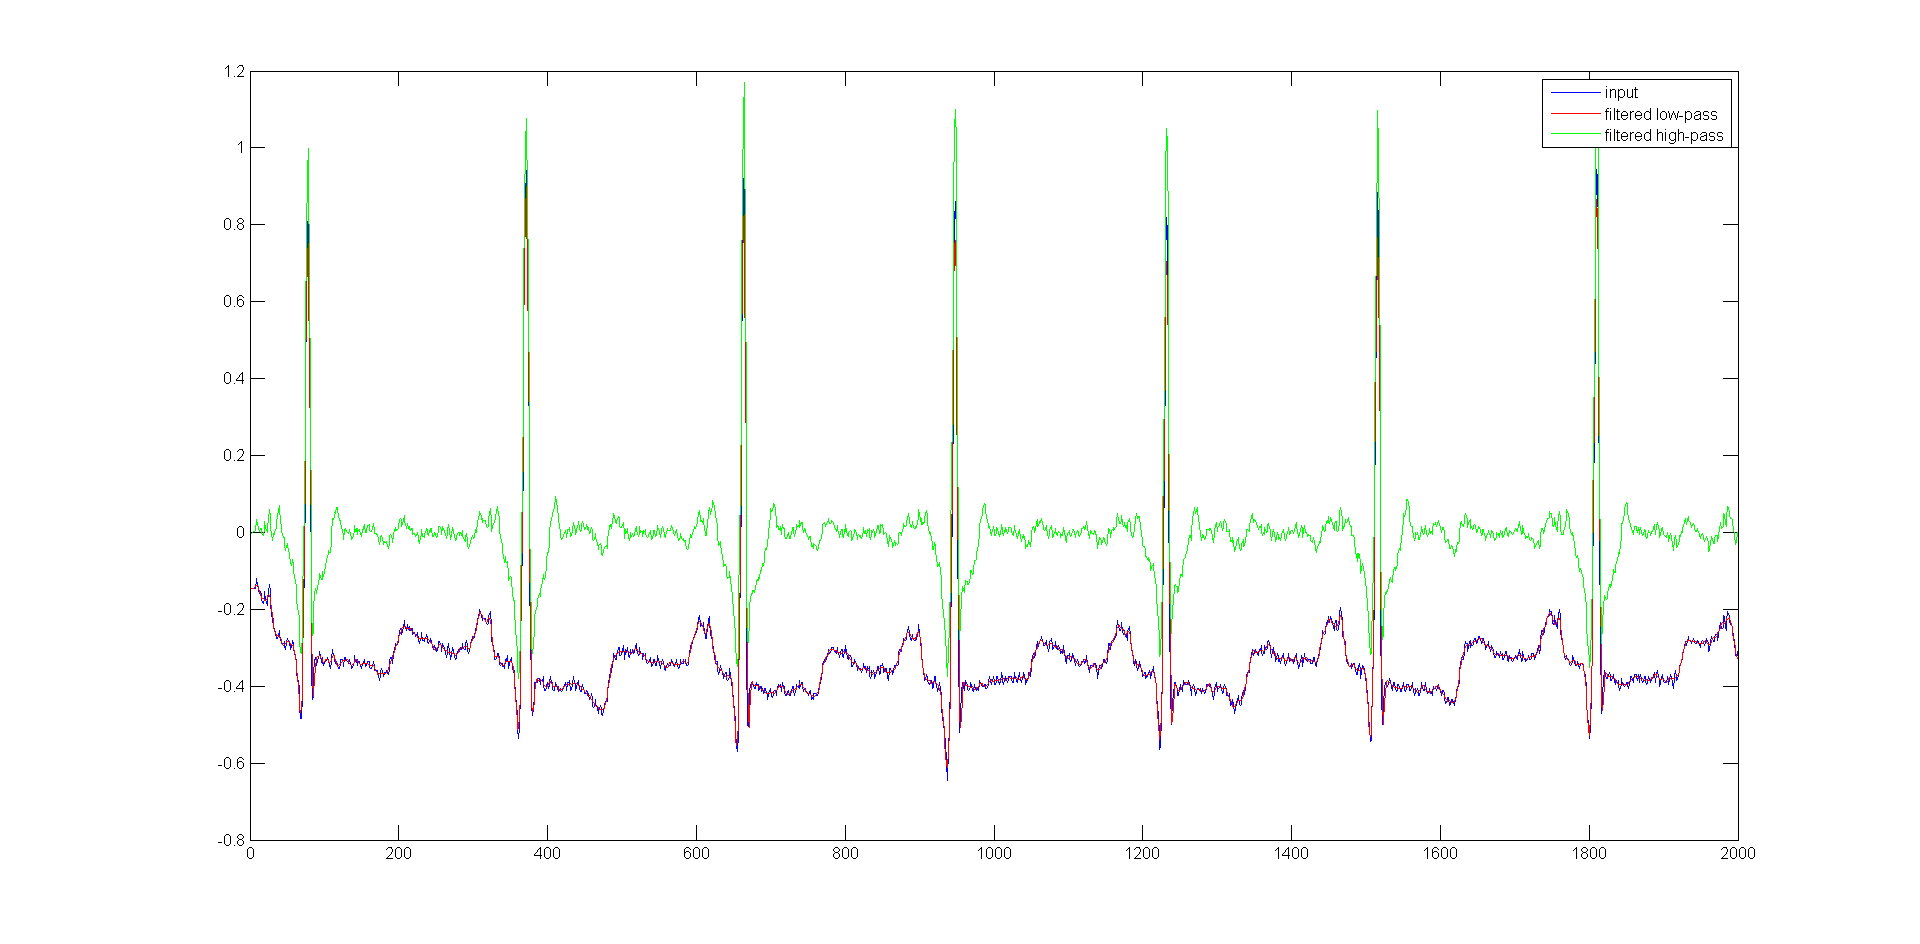
\includegraphics[width=\linewidth]{sg/filtered_by_type}
\caption{\label{sg/filtered_by_type} Rezultaty po poszczególnych etapach filtracji dla sygnału \textit{100.dat}.}
\end{figure}

Rysunek \ref{sg/final_filtered} przedstawia rezultat następujących po sobie filtracji dolno- i górnoprzepustowej. Linia bazowa sygnału jest wyrównana do wartości zera, nie występują również zakłócenia obserwowane w sygnale oryginalnym. Weryfikacja jakości wykonanego filtru została przeprowadzona w punkcie \ref{sec/tests}.

\begin{figure}[H]
\centering
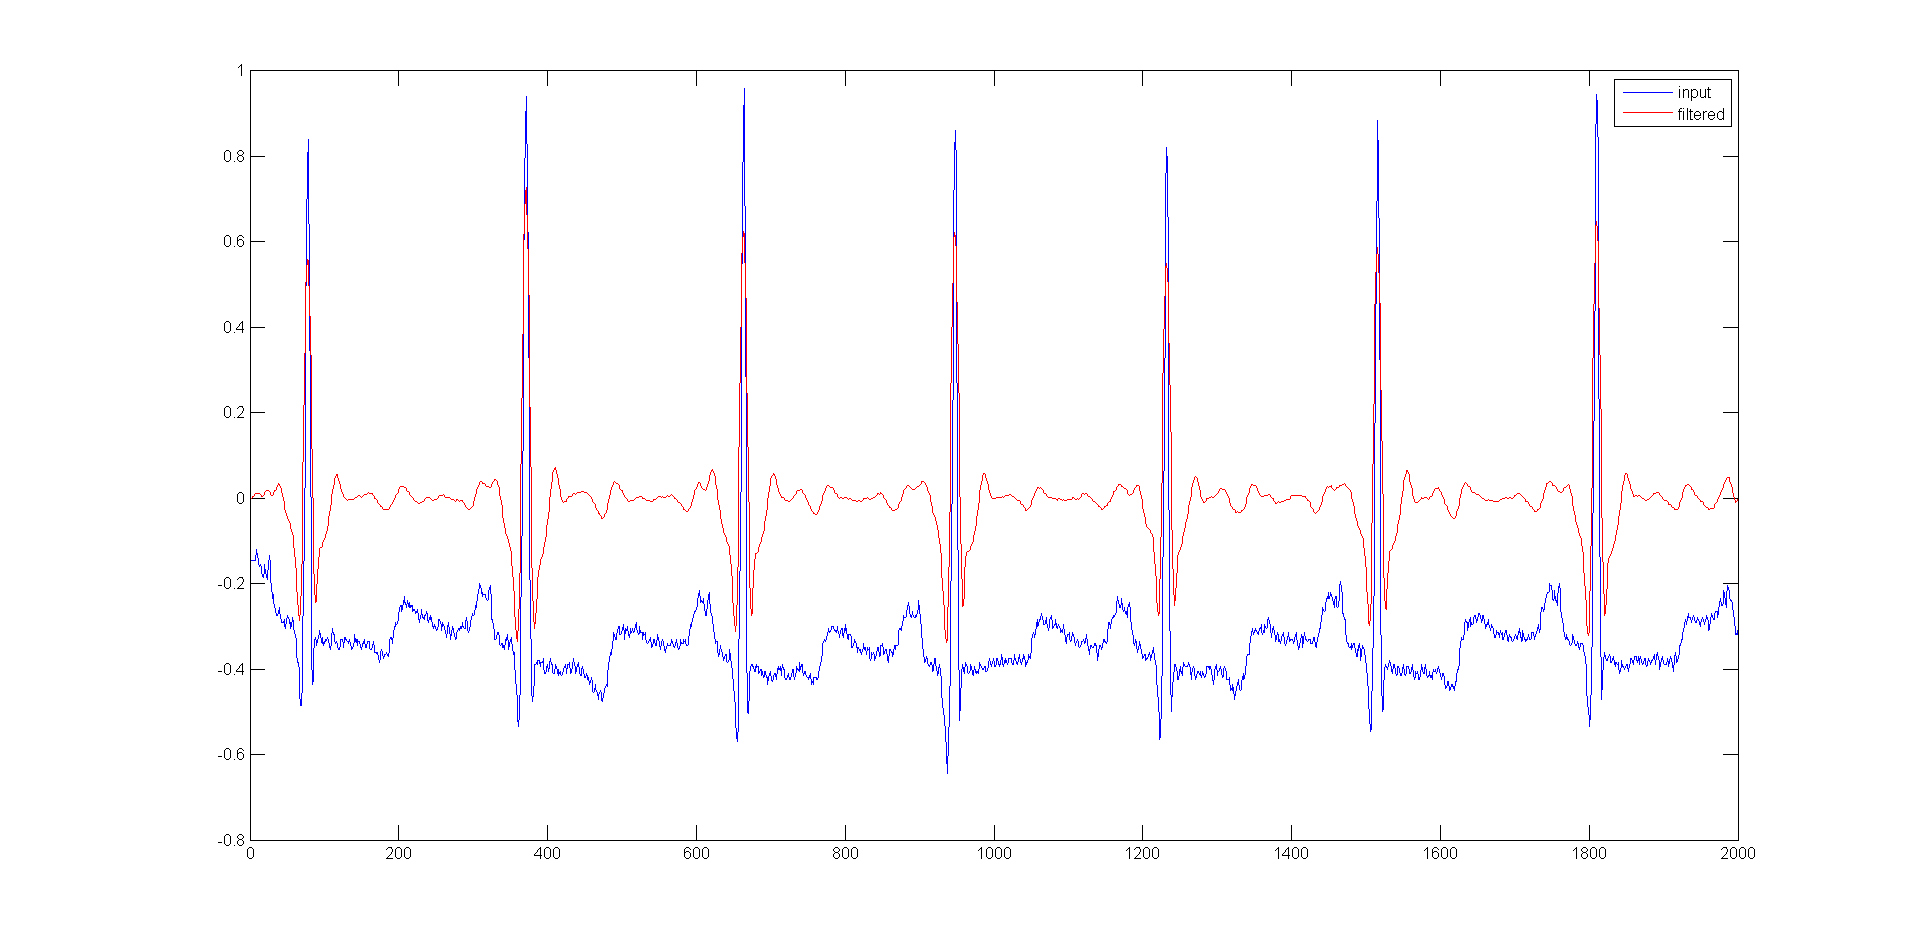
\includegraphics[width=\linewidth]{sg/filtered}
\caption{\label{sg/final_filtered} Rezultat kaskadowej filtracji dolno- i górnoprzepustowej dla sygnału \textit{100.dat}.}
\end{figure}


%%%%%%%%%%%%%%%%%%%%%%%%%%%%%%%%%%%%% END SG %%%%%%%%%%%%%%%%%%%%%%%%%%%%%%%%%%%%%%%%%


%%%%%%%%%%%%%%%%%%%%%%%%%%%%%%%%%%%%% BEGINNING NLM %%%%%%%%%%%%%%%%%%%%%%%%%%%%%%%%%%%%%%%%%%%%%%%
\subsection{Nonlocal Means}
\subsubsection{Wstęp}

Algorytm Nonlocal Means najczęściej stosowany jest w przetwarzaniu obrazów. W odróżnieniu od filtrów wykorzystujących algorytm local means, gdzie przetworzona wartość piksela liczona jest jako średnia pikseli ją otaczających to w algorytmie nonloclal means wartość piksela wyznaczana jest jako średnia ze wszystkich punktów obrazu z uwzględnieniem wagi podobieństwa pikseli w zależności od przetwarzanego punktu. 

Ten algorytm może być też stosowany do przetwarzania sygnałów 1D, co pozwala na zastosowanie go do filtracji sygnału EKG.
\subsubsection{Opis matematyczny}

\paragraph{Algorytm Nonlocal Means}
\subparagraph{}

Dla sygnału $v$, który jest oryginalnym, zaszumionym sygnałem, wartość przetworzonego sygnału $u$ wyraża się wzorem:

\begin{equation}\label{eq13}
\begin{split}
\frac{1}{Z(s)}\displaystyle\sum_{t\in{N(s)}}w(s,t)v(t),
\end{split}
\end{equation}
gdzie $w(s,T)$ są wagami, które mierzą podobieństwo pomiędzy dwoma kwadratowymi wycentrowanymi obszarami wokół $s$ oraz $t$. Wagi można zdefiniować przy pomocy równania nr \ref{eq14}.  $Z(s)$ jest znormalizowaną stałą, gdzie dla każdego $s$ zachodzi zależność $Z(s) = \sum_{t\in{N(s)}}w(s,t)$. $N(s)$ odpowiada otoczeniu punktu $s$, nazywanym często obszarem okna poszukiwań. 

\begin{equation}\label{eq14}
\begin{split}
w(s,t) = g_{h}(\displaystyle\sum_{\delta\in{\Delta}}G_{\sigma}(\delta)(v(s+\delta) - v(t+\delta))^2),
\end{split}
\end{equation}
$G_{\sigma}$ jest Gaussowskim jądrem przekształcenia wariancji $\sigma^2$, $g_{h}$ jest ciągłą nierosnącą funkcją dla której $g_{h}(0) = 1$ a $lim_{x\to+\infty}g_{h}(x) = 0$, a $\Delta$ reprezentuje obszar zawierający otoczenie punktu $\delta$.

Podsumowując algorytm Nonlocal Means odtwarza sygnał poprzez przeprowadzenie ważonej średniej wartości punktów uwzględniając przestrzenne podobieństwo pomiędzy punktami. Podobieństwo jest liczone pomiędzy równymi obszarami, w których uchwycona jest lokalna struktura (geometria, tekstura). Należy zwrócić uwagę, że punkty poza obszarem $N(s)$ nie mają wpływu na wartość $u(s)$.
Zakładamy, że okna poszukiwań $N$ i obszary $\Delta$ mają taką samą liczebność $(2K+1)^d$ i $(2P+1)^d$ dla $N = [-K,K]^d$ i $\Delta = [-P,P]^d$. 

W przedstawionym do tej pory opisie znalazły się parametry, za pomocą których wykonano odszumianie przebiegu EKG. Jednym z nich jest bazowy parametr opisany jako połowa długości $P$, czyli połowa szerokości załamka $P$ o największej amplitudzie.

Sygnałowi poddawanemu analizie odpowiada parametr $N(s)$\cite{darbon}\cite{tracey}.

\paragraph{Algorytm Fast Nonlocal Means}
\subparagraph{}

 Algorytm NLM jest dosyć skomplikowany, w związku z czym podjęto wiele starań, aby przyspieszyć jego działanie. Najczęściej stosowanym podejściem jest Fast Nonlocal Means Algorytm, zaproponowany przez Darbona. To podejście znacząco przyspiesza działanie algorytmu poprzez zmianę kolejności operacji tak aby wyeliminować zagnieżdżone pętle. Dzięki temu sygnał 1D o długości $N$ będzie mieć złożoność obliczeniową równą $O(2NM)$, podczas gdy przy tradycjonalnym podejściu wynosi $O(L_{\Delta}NM)$.

Podstawowym elementem algorytmu FNL jest efektywne policzenie wag $w(s,t)$. Wyznaczenie wag jest najbardziej czasochłonnym krokiem przy generowaniu przetworzonego sygnału $u$. Przy podejściu 1D zakładamy, że $\Omega = [0,n-1]$ dla sygnału $n$ elementowego. 
Mając wektor translacji $d_{x}$ wprowadzamy nowy sygnał $S_{d_{x}}$ jako:
\begin{equation}\label{eq15}
\begin{split}
S_{d_{x}}(p) = \displaystyle\sum_{k=0}^{p}(v(k)-v(k+d_{x}))^2 , p\in{\Omega}
\end{split}
\end{equation}

$S_{d_{x}} $ odpowiada dyskretnemu całkowaniu kwadratu różnic pomiędzy sygnałem $v$ a jego przesunięciem o wektor $d_{x}$. W sygnałach 1D mamy obszary $\Delta = [-P,P]$. Jądro przekształcenia Gaussowskiego zamienia się na stałą, co nie ma zauważalnego wpływu na sygnał, dzięki czemu równanie \ref{eq14} można zapisać w postaci: $w(s,t) = g_{h}(\sum_{\delta\in{\Delta}}(v(s+\delta_{x}) - v(t+\delta_{x}))^2)$. Zakładając, że $d_{x} = (t-s)$, a $p=s+\delta_{x}$ to równanie $w(s,t)$ można przeparametryzować do postaci $w(s,t) = g_{h}(\sum_{p=s-P}^{s+P}(v(p) - v(p+d_{x}))^2)$. Jeżeli rozdzielimy sumę i użyjemy równania nr \ref{eq15} to uzyskamy: 

\begin{equation}\label{eq16}
\begin{split}ł
w(s,t) = g_{h}(S_{d_{x}}(s+P)-S_{d_{x}}(s-P))
\end{split}
\end{equation}
Równanie nr \ref{eq16} jest niezależne od t z założeniem, że wielkość $S_{d_{x}}$ jest znana. Jest to kluczowe równanie, które pozwala na wyznaczenie wag dla pary punktów w stałym czasie. 

Podsumowując, działanie algorytmu można opisać jako  wyznaczenie wartości $S_{d_{x}}$ z wykorzystaniem równania \ref{eq15}, następnie wyznaczane są wagi korzystając z równania \ref{eq14} i \ref{eq16}, a na koniec przeprowadzana jest filtracja na podstawie równania \ref{eq13}. Procedura jest powtarzana dla wszystkich możliwych translacji wyznaczonych przez wymiar okna poszukiwań $N$\cite{darbon}\cite{tracey}.
 
\subsubsection{Implementacja algorytmu}

\begin{algorithm}
\caption{Algorytm Fast-NLM }
\begin{algorithmic}[1]
\Input $v,K,P,h$
\Output $u$
\Temporary $S_{d_{x}}, Z, M$
\State Inicjalizacja $u$, $M$, $Z$ jako $0$.
\ForAll{$d_{x}\in[-K,K]$}
\State {Obliczenie $S_{d_{x}}$ na podstawie równania \ref{eq15}}
\ForAll {$s\in[0,n-1] $}
\State {Obliczenie wag w na podstawie równania \ref{eq14} i \ref{eq16}}
\State {$u(s)\leftarrow u(s) + w\cdot u(s+d_{x})$}
\State{$M(s) = max(M(s),w)$}
\State {$Z(s)\leftarrow Z(s) + w$}
\EndFor
\EndFor
\ForAll {$s\in[0,n-1] $}
\State {$u(s)\leftarrow u(s) + M(s) \cdot v(s)$}
\State {Zastosowanie normalizacji sygnału wyjściowego}
\State {$u(s)\leftarrow \frac{u(s)}{Z(s) + M(s)} $}
\EndFor
\State \textbf{return} $u$
\end{algorithmic}
\end{algorithm}

Do implementacji algorytmu zostały użyte 4 parametry wejściowe, oznaczone kolejno jako $v$, $K$, $P$ oraz $h$. Symbolem $v$ oznaczono sygnał wejściowy, podawany na wejście implementowanej funkcji. Użyty  parametr $h$, decydował o stopniu wygładzenia sygnału po filtracji. Zbyt mała wartość tego parametru oznacza zbyt duży wpływ szumu, co skutkuje niedostatecznym uśrednianiem sygnału. Efektem przyjęcia za parametr $h$ zbyt dużej wartości jest zmiana wyglądu przebiegów sygnału EKG, która spowoduje że wiele sygnałów będzie do siebie podobnych mimo występujących różnic. Pierwszy z dwóch kolejnych parametrów- $K$, został wykorzystany do stworzenia wektora będącego zbiorem według którego iterowane były kolejne przejścia algorytmu. Parametr $P$ odpowiadał natomiast za sąsiedztwo w którym wyszukiwane będą kolejne próbki. Odpowiedni dobór zakresu sąsiedztwa wpływa m.in. na szybkość przeszukiwania sygnału co ma bezpośredni wpływ na wydajność algorytmu. Zbyt duży zakres sąsiedztwa sprawi, że czas kompilacji zostanie wydłużony, nawet w przypadku szybkiego algorytmu. Dobór odpowiednio dużego $P$ umożliwi porównanie ze sobą zespołów QRS występujących w zakresie parametru $P$\cite{tracey}.

\subsubsection{Rezultaty}

Filtracja zrealizowanym filtrem NLM pozwoliła w efektywny sposób usunąć zakłócenia sygnału. Przefiltrowany sygnał nie oddaje w pełni przebiegu surowego sygnału. Skutkuje to wyraźnym spłaszczeniem linii sygnału pomiędzy kolejnymi zespołami QRS, przy jednoczesnym zachowaniu załamków P i T. Przyjęte parametry filtru mają istotne znaczenie przy optymalizacji jego działania. Odpowiedni dobór szerokości zakresu poszukiwań, w tym przypadku było to 500 próbek pozwolił na zrealizowanie optymalnej filtracji. Na Rys. \ref{nlm/zestawienie2} pokazano rezultat działania zaimplementowanego filtru NLM.

\begin{figure}[H]
\centering
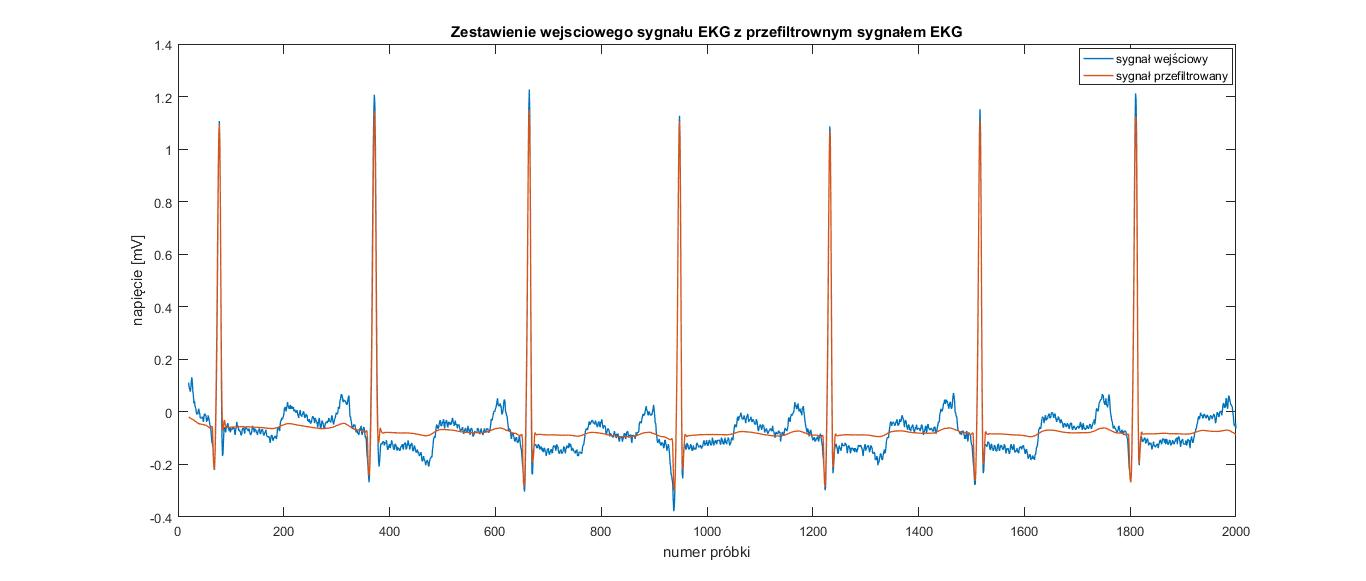
\includegraphics[width=\linewidth]{nlm/zestawienie2}
\caption{\label{nlm/zestawienie2}  Rezultat filtracji filtrem Nonlocal Means.}
\end{figure}

%%%%%%%%%%%%%%%%%%%%%%%%%%%%%%%%%%%%%%%% END NLM %%%%%%%%%%%%%%%%%%%%%%%%%%%%%%%%%%%%%%%%%%%%%%%%%%

%%%%%%%%%%%%%%%%%%%%%%% WWF %%%%%%%%%%%%%%%%%%%%%%%%%%%%%%%%

\subsection{Dekompozycja falkowa z użyciem filtra Wienera}

Sygnał elektrokardiograficzny, będący zapisem aktywności elektrycznej serca, można traktować jako kombinację sygnału właściwego oraz zakłóceń. Głównym źródłem zakłóceń w zapisie EKG są potencjały elektryczne pochodzenia mięśniowego (EMG), zawierające się w szerokim paśmie częstotliwości. Ponieważ zakresy częstotliwości obu sygnałów (EKG i EMG) nachodzą na siebie, filtracja pasmowo-zaporowa sygnałów mięśniowych powoduje zniekształcenie sygnału elektrokardiograficznego, szczególnie zespołów QRS. Alternatywną metodą usuwania zakłóceń może być zastosowanie transformacji falkowej. W wyniku prostej transformacji falkowej można w pasmach najwyższej częstotliwości wyodrębnić zakłócenia wraz z pewnymi składowymi zespołów QRS \cite{smital}. Zasadnicza część składowych QRS znajduje się w pasmach niższych częstotliwości. Sygnał wynikowy można filtrować poprzez dopasowywanie współczynników transformacji. 

\subsubsection{Opis metody - progowanie w dziedzinie falek}

Proste filtry falkowe są oparte o dopasowywanie współczynników transformacji falkowej. W przypadku filtracji EKG można zastosować oddzielanie sygnału właściwego oraz zakłóceń metodą progowania. Należy przy tym wybrać rodzaj progowania oraz wartość progu. 

Załóżmy, że zakłócony sygnał $x(n)$ jest sumą czystego sygnału $s(n)$ oraz zakłóceń $w(n)$:

\begin{equation} 
x(n) = s(n)+w(n)
\end{equation}

przy czym, sygnał i zakłócenia nie są wzajemnie skorelowane. Jeśli przeprowadzimy transformację sygnału do dziedziny falek przy użyciu stacjonarnego przekształcenia falkowego, otrzymamy współczynniki falek:

\begin{equation} 
y_m (n)=u_m (n)+v_m (n)
\end{equation}

Gdzie: 
$u_m(n)$ – współczynniki właściwego sygnału
$v_m (n)$ – współczynniki zakłóceń
$m$ – stopień dekompozycji, (m-te pasmo częstotliwości).

Wartości progów stosowanych do modyfikacji współczynników falek powinny być ustalane osobno dla każdego stopnia dekompozycji $m$, w zależności od odchylenia standardowego sygnału $v_m (n)$ (czyli $\sigma_vm$). Do wyznaczania wartości progu używamy odchylenia standardowego sygnału zakłóceń pomnożonego przez empirycznie wyznaczoną stałą, $TM$. Wartości progów można opisać równaniem:

\begin{equation} 
\lambda_m = TM \times \sigma_vm
\end{equation}

gdzie $\sigma_vm$ jest odchyleniem standardowym sygnału zakłóceń w m-tym paśmie częstotliwości.

\subsubsection{Filtracja metodą Wienera}

Posiadając współczynniki $y_m (n)$ jesteśmy w stanie oszacować współczynniki właściwego sygnału $u_m (n)$ za pomocą metody Wienera zastosowanej w dziedzinie falek. Metoda ta jest przedstawiona na rys. \ref{wwf/WWF_diagram}.

\begin{figure}[H]
\centering
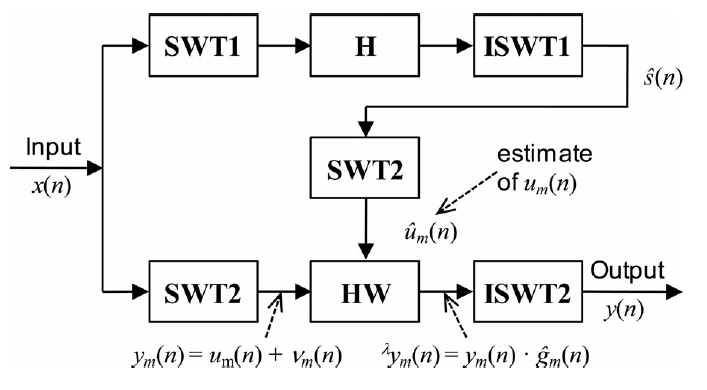
\includegraphics[width=0.6\textwidth]{wwf/WWF_diagram}
\caption{\label{wwf/WWF_diagram} Idea filtracji metodą Wienera w dziedzinie falek.}
\end{figure}

Przy użyciu odwrotnej transformacji falkowej ISWT1 jesteśmy w stanie oszacować $\check{s}(n)$, co w przybliżeniu stanowi szukany sygnał bez zakłóceń. To przybliżenie jest używane do zaprojektowania filtra Wienera $(HW)$, który jest stosowany do oryginalnego sygnału z zakłóceniami $x(n)$ w dziedzinie SWT2, z użyciem współczynnika korekcji Wienera:


\begin{equation} 
\check{g}_m(n)=\frac{\check{u}^2_m(n)}{\check{u}^2_m(n)+\sigma^2_m(n)}
\end{equation}

Gdzie:
$\check{u}^2_m(n)$– współczynniki falek uzyskane z przybliżenia $\check{s}(n)$,
$\sigma^2_m(n)$ – wariancja współczynników sygnału zakłóceń $v_m (n)$ w paśmie $m$.

W bloku HW przetwarzamy współczynniki sygnału z zakłóceniami $y_m (n)$ przy użyciu współczynnika korekcji Wienera, w celu uzyskania zmodyfikowanych współczynników:

\begin{equation} 
y^\lambda_m (n)=y_m (n) \times \check{g}_m(n)
\end{equation}

Sygnał wyjściowy $y(n)$ uzyskiwany jest w drodze odwrotnej transformacji ISWT2 zmodyfikowanych współczynników $y^\lambda_m (n)$.

\subsubsection{Implementacja}

Implementacja algorytmu podzielona została na następujące etapy:
	
\begin{enumerate}
\item Usunięcie składowej stałej sygnału, oszacowanej na podstawie mediany. 
\item Transformacja falkowa czwartego stopnia falką z rodziny bior2.2 w bloku SWT1.
\item Wyznaczenie wartości progu dla każdego poziomu dekompozycji za pomocą estymaty odchylenia standardowego. Dla każdego poziomu dekompozycji estymatę wyznaczono osobno z następującej zależności:

\begin{equation} 
\sigma_vm=\frac{median(y_m)}{0,6745}
\end{equation}

\item Progowanie sygnału w dziedzinie falek funkcją typu Garrote, z progiem $3 \sigma_vm$.
\item Obliczenie estymaty sygnału niezaszumionego poprzez odwrotną transformację falkową sprogowanego sygnału.
\item Filtracja sygnału w przestrzeni falkowej za pomocą filtru Wienera, z wykorzystaniem wyznaczonej estymaty. 
\item Odwrotna transformacja falkowa, w celu uzyskania sygnału w dziedzinie próbek.
\end{enumerate}

\subsubsection{Rezultaty}
	
Filtracja sygnału przy pomocy dekompozycji falkowej oraz filtracji Wienera dała specyficzny rodzaj rezultatu, w którym zakłócenia o wysokich częstotliwościach zostały usunięte, jednak amplituda zespołów QRS nie uległa zmniejszeniu, nie zostały one również poszerzone. Można zatem stwierdzić, że udało się osiągnąć efekt selektywnej filtracji w dziedzinie wysokich częstotliwości. Jednocześnie w okresach pomiędzy poszczególnymi zespołami QRS zaobserwowano spłaszczenie załamków P i T. Uzyskany sygnał wyjściowy nie stanowi wiernego odtworzenia sygnału poddawanego filtracji, jednak posiada cechę silnego uwydatnienia zespołów QRS, co może stanowić duże ułatwienie w ich detekcji.
    
\begin{figure}[H]
\centering
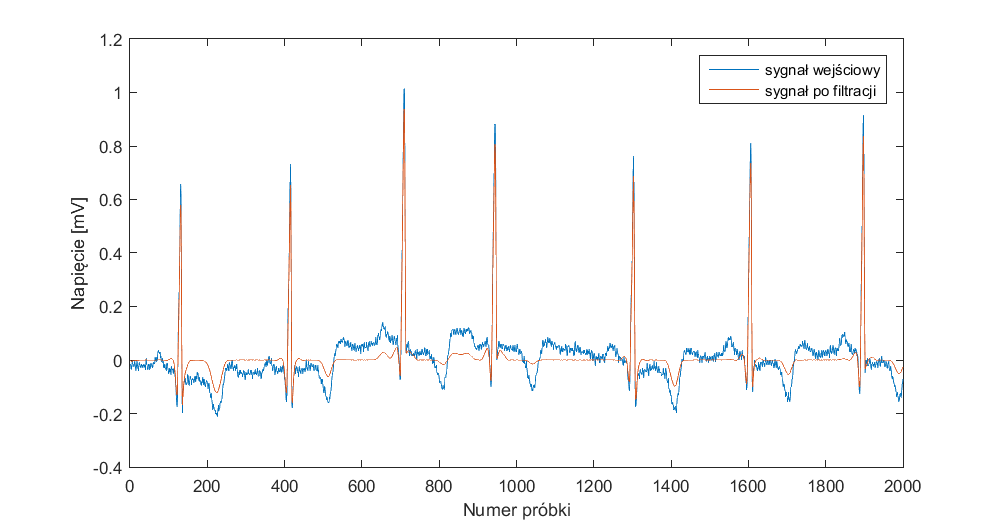
\includegraphics[width=1\textwidth]{wwf/wynik}
\caption{\label{wwf/wynik} Wynik filtracji sygnału $100.dat
$ metodą Wienera w dziedzinie falek.}
\end{figure}

%%%%%%%%%%%%%%%%%%%%%%%%%%%%%%%%%%%%%%%% EMD START %%%%%%%%%%%%%%%%%%%%%%%%%%%%%%%%%%%%%%%%%%%%%%%%%%
\subsection{ECG denoising - Empirical mode decomposition}
Celem tej części jest opracowanie, implementacja i przeprowadzenie testów algorytmu filtracji sygnału EKG z wykorzystaniem metody empirycznej dekompozycji (\textit {ang. Empirical mode decomposition}) w środowisku C++. Prace nad algorytmem zostały podzielone na główne składowe, z których ten raport obejmuje: 
\begin{itemize}
	\item projekt toru przetwarzania sygnału
	\item wstępna implementacja algorytmu z wykorzystaniem środowiska Matlab i jego testowanie
\end{itemize}

\subsubsection{Opis metody - algorytmu}
Dekompozycja empiryczna należy do czasowo-częstotliwościowej transformaty sygnału, z której bazą jest sam analizowany sygnał. Ogólna zasada działania algorytmu polega na założeniu, że każdy sygnał zawiera w sobie różne proste oscylacje - funkcje składowe IMF (\textit {ang. intrinsic mode function}). Funkcje te spełniają następujące warunki: 

\begin{enumerate}
	\item Maksymalna różnica pomiędzy ilością ekstremów a przejść przez zero jest równa 1.
	\item W dowolnym punkcie średnia wartość obwiedni utworzonej przez maksima i minima musi być równa 0.
\end{enumerate}

W celu uzyskania składowych IMF z oryginalnego sygnału należy przeprowadzić na nim następujące działania: 

\begin{enumerate}
	\item Identyfikacja wszystkich maksimów i minimów. 
	\item Przeprowadzenie interpolacji  w celu uzyskania górnej (dla maksimów) i dolnej (dla minimów) obwiedni. równa 0.
	\item Obliczenie średniej pomiędzy dwiema obwiedniami i odjęcie jej od sygnału w celu wyodrębnienia detali

\begin{equation} 
  x_{avg}(t) = \frac{x_{min}(t) +x_{max}(t)}{2}
 \end{equation}
\begin{equation}
  d_{k-1}(t) = x(t) - x_{avg}(t)
 \end{equation}
Gdzie:
\begin{itemize}
	\item[] 
	\begin{itemize}
	 	\item[] $d_{k-1}(t)$ - sygnał wejściowy dla kolejnej iteracji
		\item[] $x_{min}(t)$ - minimum
		\item[] $x_{max}(t)$ - maksimum
	\end{itemize}
\end{itemize}

	\item Jeśli wyznaczona składowa spełnia warunki 1-2 to dokonuje się jej ekstrakcji z oryginalnego sygnału uzyskując sygnał resztkowy. W przypadku gdy wyznaczona składowa nie spełnia kryteriów koniecznym jest powtórzenie poprzednich kroków do momentu aż zacznie je spełniać.

\begin{equation} 
  r_{1}(t) = x(t) +d_{k}(t)
 \end{equation}
\begin{equation}
  h_{1}(t) = d_{k}(t)
 \end{equation}

Gdzie:
\begin{itemize}
	\item[] 
	\begin{itemize}
	 	\item[] $r_{1}(t)$ - sygnał który bierze udział w wyznaczaniu kolejnego IMF
		\item[] $x(t)$ - sygnał oryginalny
		\item[] $d_{k}(t)$ - pierwszy z IMF
		\item[] $h_{1}(t)$ - sygnał resztkowy pierwszej iteracji
	\end{itemize}
\end{itemize}

	\item Traktując uzyskany sygnał resztkowy jako sygnał analizowany powtarza się poprzednie kroki w celu wyznaczenia kolejnej funkcji składowej IMF
\end{enumerate}

Proces dekompozycji zostaje zakończony w momencie gdy nie jest możliwym wyodrębnienie kolejnych IMF z analizowanego sygnału, gdy komponenty IMF niosą w sobie wystarczającą informacje o amplitudzie i modulacji sygnału. W takiej sytuacji analizowany sygnał jest funkcją monotoniczną bądź stałą. Dodatkowym kryterium zakończenia dekompozycji jest odchylenie standardowe pomiędzy kolejnymi sygnałami resztkowymi uzyskiwanymi podczas procesu dekompozycji. Typowo parametr SD przyjmuje zakres wartości $0.2 - 0.3$.

\begin{equation}
	SD=\sum_{t=0}^{L-1} \bigg[\frac{|d_{k-1}(t)-d_{k}(t)|^{2}}{d_{k-1}^{2}(t)}\bigg]
 \end{equation}

Proponowana metoda wykorzystania EMD w filtracji sygnału EKG ma polegać na przeprowadzeniu filtracji IMF zdominowanych przez szum. Przyjęto za zaszumione trzy pierwsze IMF \cite{1}, a następnie poddano je po zsumowaniu filtracji przy pomocy filtru IIR Butterwortha.
Po przeprowadzonej filtracji sygnał jest rekonstruowany: 

\begin{equation}
	\hat{x}(t) = \sum_{k=1}^{n} \tilde{h}_{k}(t) + \sum_{k=n+1}^{N}h_{k}(t)+r_{N}(t)
 \end{equation}

Gdzie:
\begin{itemize}
	\item[] 
	\begin{itemize}
	 	\item[] $\tilde{h}_{k}(t)$ - przefiltrowana wersja $h_{k}(t)$
		\item[] $r_{N}(t)$ - pozostały sygnał IMF
	\end{itemize}
\end{itemize}

\subsubsection{Działanie algorytmu}
Algorytm zaimplementowany został zgodnie ze schematem podanym we wstępie. Jako środowisko wybrany do stworzenia prototypu został program Matlab, ze względu na dużą ilość już wbudowanych funkcji, które mogą być wykorzystane.Ostateczna wersja została napisana w języku C++, z wykorzystaniem biblioteki Eigen. W proponowanym algorytmie proces rozpoczyna się od dekompozycji, gdzie wyszukiwane są kolejne komponenty IMF. Zgodnie z \cite{2}, dla każdej wyznaczonej funkcji, mogącej być funkcją oscylacyjną, sprawdzane są warunki (2.3.1). Jeżeli w kolejnych iteracjach, nie dojdzie do znalezienia odpowiedniego komponentu IMF, jest on wyznaczany jako funkcja, dla której SD, pomiędzy nią, a tą z poprzedniej iteracji, jest mniejsze niż 0,3.  Przyjęta wartość progowa, jest wynikiem licznych prób algorytmu, dając najlepsze rezultaty. Źródła \cite{1}, podają jej wartość jako przedział 0,2-0,3, co jednak w praktyce dało gorsze wyniki.  Sam proces przesiewania może się więc zakończyć w następujących przypadkach:
\begin{itemize}
  \item Znalezienie imf, spełniającej kryteria
  \item Znalezienie imf, wyznaczoną na podstawie SD
  \item Brak możliwości wygenerowania obwiedni sygnału (na podstawie minimów i maksimów), ze względu na niewystarczającą ilość punktów (minimum 2)
\end{itemize}
Ostatni warunek, wynika z faktu, iż w kolejnych iteracjach analizowany sygnał zmienia się, zgodnie ze wzorami 19 i 20. 
Proces zostaje zakończony, gdy  r  przestaje być funkcją monotoniczną, co powoduje,   że nie można  wyodrębnić  więcej    składowych  IMF.  Rysunek \ref{emd/rawsignal}   przedstawia przykładowy sygnał EKG (sygnał nr 100 z bazy MIT-BIH Arrythmia Database), który poddany został analizie i zostanie pokazany jako przykład w tym 
raporcie.

\begin{figure}[H]
\centering
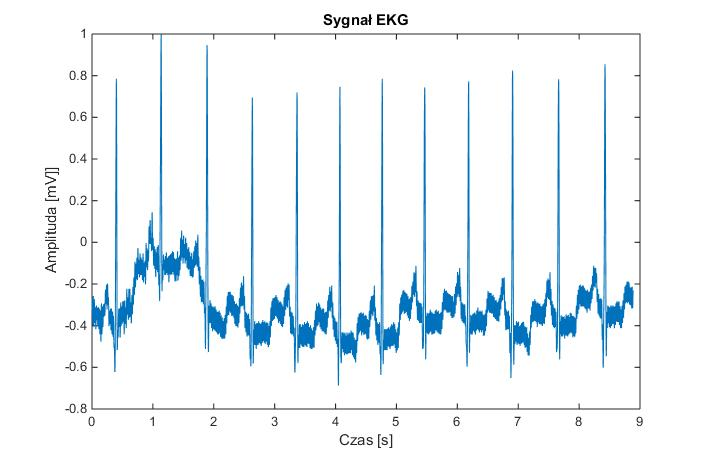
\includegraphics[scale=0.5]{emd/rawsignal}
\caption{\label{emd/rawsignal}Sygnał EKG poddawany analizie}
\end{figure}

Po dokonaniu procesu przesiewania uzyskano kolejne funkcje oscylacyjne IMF (Rysunek \ref{emd/IMFS}).  Zakłócenia sygnału w postaci szumów zawarte są w kilku pierwszych funkcjach \cite{2, 3}. Ostatecznie zastosowana metoda określania ilości zaszumionych komponentów, jest inna niż miało to miejsce w prototypie. Tam był to parametr płaskości widma (ang. Spectral Flatness- SF) dla każdej funkcji oscylacyjnej \cite{2}. Dalsza praktyka i testy, pokazały jednak, że nie jest to odpowiedni wyznacznik. Przyjmując za zaszumione te parametry, których SF jest mniejsza od stałej wartości progowej, dochodziło do sytuacji, że nie tylko kilka pierwszych funkcji oscylacyjnych zostało za takie uznane (czego można było się spodziewać, gdyż szumy są zawarte w kilku pierwszych imf), ale również taka sytuacja często miała miejsce dla tych ostatnich, które szumów teoretycznie nie powinny zawierać. Po zsumowaniu wyznaczonych funkcji i filtracji, wyniki okazały się nie być zadowalające, przede wszystkim dlatego, że znacznie malały różnice w wysokościach załamków. 
Zastosowano więc rozwiązanie prezentowane w \cite{1}, jako zaszumione uznano 3 pierwsze funkcje imf, które niosą wysokoczęstotliwościowe szumy, ale również część użytecznej informacji o sygnale. Pozostałe funkcje uznano za niosące informację użyteczną. 

\begin{figure}[H]
\centering
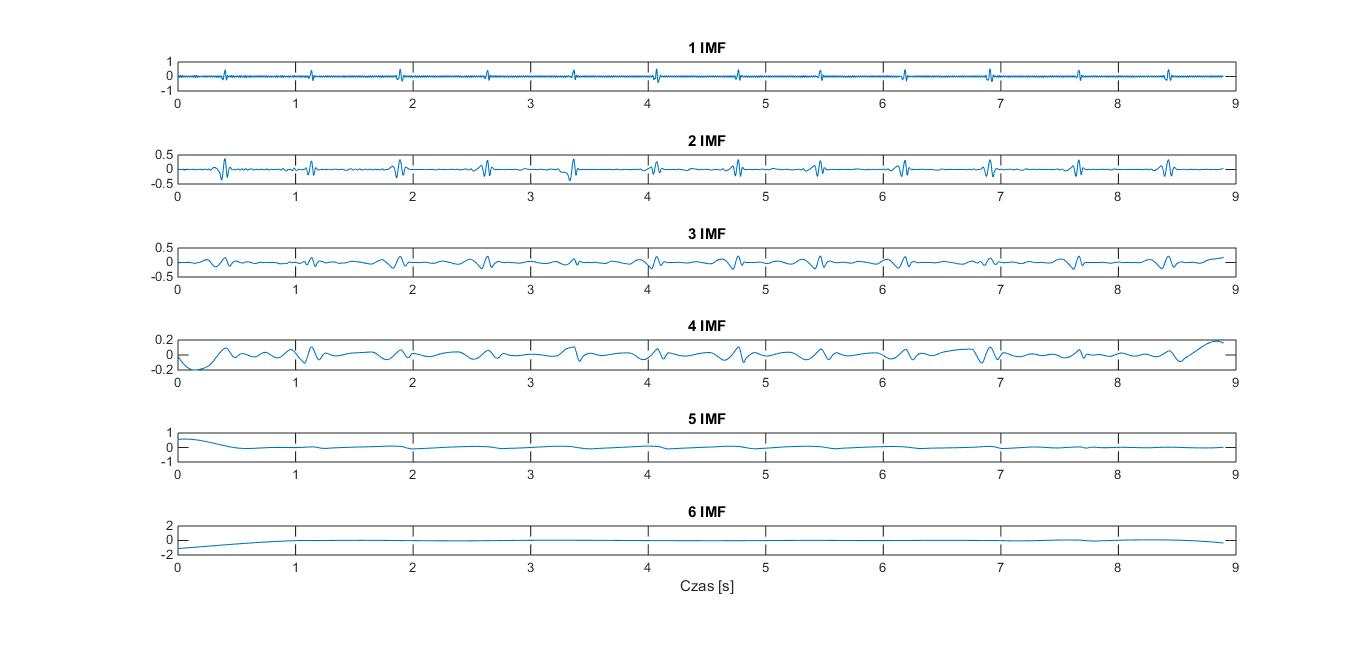
\includegraphics[scale=0.35]{emd/IMFS}
\caption{\label{emd/IMFS}Kolejne funkcje oscylacyjne sygnału EKG}
\end{figure}

Rezultatem procesu przesiewania, oprócz powyższych funkcji, był również sygnał resztkowy, czyli pozostałość wejściowego, z której nic nie można już było wyodrębnić (Rysunek \ref{emd/residue}). 


\begin{figure}[H]
\centering
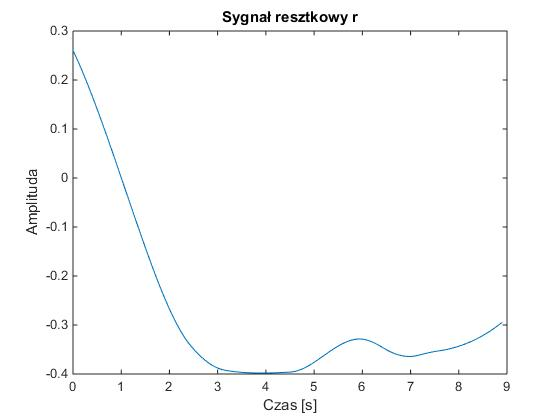
\includegraphics[scale=0.6]{emd/residue}
\caption{\label{emd/residue} Sygnał resztkowy}
\end{figure}


Kolejnym etapem było odszumienie funkcji uzyskanej jako sumę 3 pierwszych oscylacyjnych. Na tym etapie również wprowadzono modyfikacje w stosunku do prototypu, używającego filtru pasmowo-przepustowego o paśmie 5-20 Hz, zrealizowanego jako kaskadowe połączenie filtra dolno i górnoprzepustowego.
W celu przeprowadzenia operacji odszumiania, zastosowano filtr IIR Butterwortha o pasmie przepustowym 5-60 Hz (częstotliwość próbkowania wynosiła 360 Hz). Dało to zdecydowanie lepsze rezultaty w jakości wyjściowego sygnału, redukując znacznie więcej szumów. Ponadto poprzednie rozwiązanie sprawdzało się wyłącznie dla mocno zaszumionych sygnałów, natomiast nowe równie dobrze działa w przypadkach nawet słabych zakłóceń.

Rezultaty przedstawiono na Rysunkach \ref{emd/IMFnoise} i \ref{emd/IMFfilteredIIR}. Filtr, jak widać zdecydowanie poprawia jakość sygnału, zaproponowane pasmo częstotliwości, pozwala na dalszą swobodną analizę sygnału. Wcześniej filtracja była aspektem, który jak zaznaczono w raporcie cząstkowym należało udoskonalić, co można uznać zakończyło się powodzeniem. 

\begin{figure}[H]
\centering
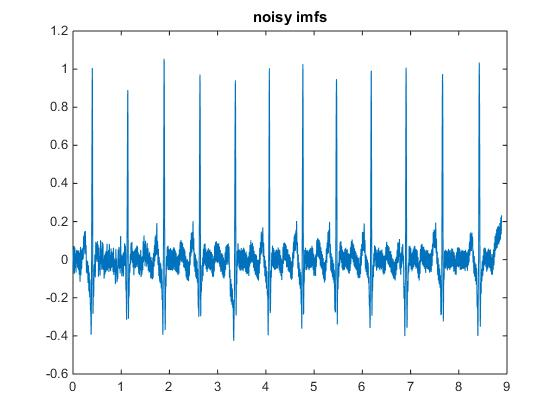
\includegraphics[scale=0.5]{emd/IMFnoise}
\caption{\label{emd/IMFnoise} Zaszumione 3 pierwsze funkcje oscylacyjna}
\end{figure}

  
\begin{figure}[H]
\centering
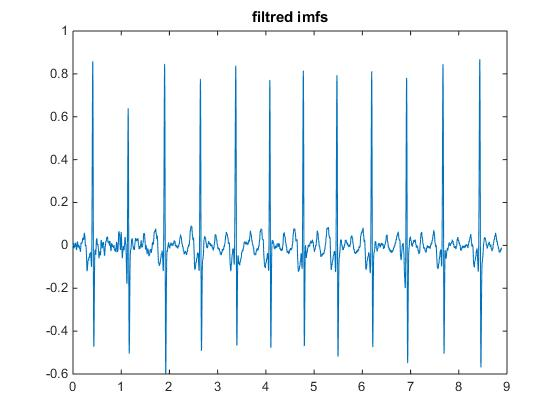
\includegraphics[scale=0.5]{emd/IMFfilteredIIR}
\caption{\label{emd/IMFfilteredIIR} Przefiltrowane 3 pierwsze funkcje oscylacyjne}
\end{figure}

Ostatecznie przefiltrowane funkcje oscylacyjne dodano do pozostałych oraz do sygnału resztkowego. Utworzony w ten sposób sygnał stanowi końcową wersję- przefiltrowany sygnał EKG (Rysunek \ref{emd/filtredECG_IIR}). 

\begin{figure}[H]
\centering
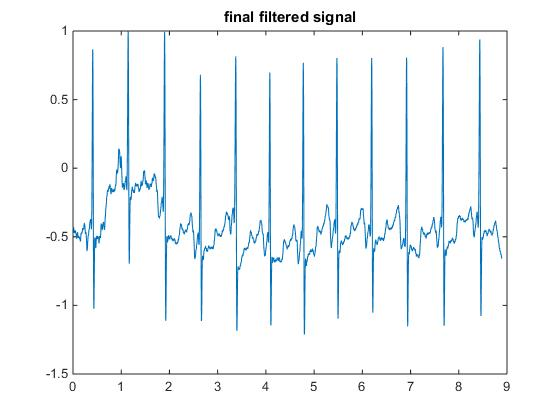
\includegraphics[scale=0.7]{emd/filtredECG_IIR}
\caption{\label{emd/filtredECG_IIR} Przefiltrowany sygnał EKG}
\end{figure}

\paragraph{Podsumowanie}
\subparagraph{}

Przedstawione w artykule wyniki eksperymentu potwierdzają możliwość zastosowania  metody EMD do filtracji sygnałów EKG oraz poprawność wykonania prototypu. Porównując sygnał wejściowy i wynikowy, widać wyraźną poprawę jakości i uzyskanie znacznej redukcji szumów. Z diagnostycznego punku widzenia może mieć to szerokie zastosowanie w dalszej analizie sygnału pod kątem występowania w nim nieprawidłowości.




%%%%%%%%%%%%%%%%%%%%%%%%%%%%%%TESTY%%%%%%%%%%%%%%%%%%%%%%%%%%%%%%%%%%%%%%%%%%%%%%%%%%%%%%%%%%%%%%%%%%%%%
\section{Testy}
\label{sec/tests}


\subsection{RMSE}

Aby móc określić jakość zaimplementowanych algorytmów należało porównać je z sygnałem uznanym za referencyjny. W tym celu użyto filtru napisanego w ramach zajęć laboratoryjnych, otrzymując tym samym dane pozwalające na porównania. Został on zbudowany jako połączenie kaskadowe filtrów: dolnoprzepustowego o częstotliwości odcięcia 60 Hz i górnoprzepustowego dla 5 Hz, częstotliwość próbkowania ustalona została na 360 Hz. Przy projektowaniu, dla każdego filtru zostało wykorzystane okno Hamminga. Wyniki zostały otrzymane dla sygnałów EKG z bazy MIT-BIH Arrhythmia Database \cite{mit-bih, mit-bih-2}. Pobrano 10 plików z rejestracji sygnału EKG. Każdy zapis zawiera 650000 próbek rejestrowanych z częstotliwością 360 Hz . Surowe sygnały EKG, które zostały wykorzystane podczas testów, znajdują się w następujących plikach:
100.dat, 101.dat, 102.dat, 103.dat, 104.dat, 105.dat, 106.dat, 107.dat, 108.dat, 109.dat.
Każdy z tych sygnałów po przefiltrowaniu stał się wzorem, względem którego wyznaczono parametry jakościowe dla innych metod filtracji, dla analogicznych danych.

Pierwiastki błędu średniokwadratowego dla zaimplementowanych filtrów obliczone względem sygnału referencyjnego zestawiono w tabeli \ref{rmse}.

\setcounter{rownum}{99}
\begin{table}[H]
\centering
\caption{\label{rmse} Współczynnik RMSE dla sygnałów przefiltrowanych różnymi filtrami.}
  \begin{tabular}{lrrr R{0.2\linewidth}}
  \toprule
      Sygnał			& Savitzky-Golay	& Nonlocal Means	& Wavelet Wiener*	& Empirical Mode Decomposition	\\
  \midrule
  \midrule
      \rownum.dat 		& 0,1602			& 0,0792		& 0,1084   	& 0,1318    	\\
      \rownum.dat 		& 0,1788         	& 0,1248		& 0,1282   	& 0,1049    	\\
      \rownum.dat 		& 0,0954         	& 0,0836		& 0,1193   	& 0,1412    	\\
      \rownum.dat 		& 0,2509         	& 0,1288		& 0,1557   	& 0,1090    	\\
      \rownum.dat 		& 0,1460          	& 0,1065		& 0,1466   	& 0,1353    	\\
      \rownum.dat 		& 0,2238         	& 0,2072		& 0,2157   	& 0,1144    	\\
	  \rownum.dat 		& 0,2480         	& 0,1541		& 0,1881   	& 0,1467    	\\
      \rownum.dat 		& 0,3750         	& 0,3923		& 0,6555   	& 0,2269    	\\
      \rownum.dat 		& 0,1242         	& 0,1941		& 0,1300   	& 0,1143    	\\
      \rownum.dat 		& 0,3185         	& 0,1876		& 0,3406   	& 0,1572    	\\
  \midrule
      średnia 			& 0,2121           	& 0,1658		& 0,2188   	& 0,1382    	\\
  \bottomrule 
  \end{tabular}
\end{table}
\setcounter{rownum}{0}
\FloatBarrier
* Wyniki dla filtra Wavelet Wiener zostały uzyskane na podstawie implementacji w środowisku MATLAB.

\subsection{Czas filtracji}

Czasy osiągane przez zaimplementowane w ramach projektu algorytmy zestawiono w tabeli \ref{time}. 

\setcounter{rownum}{99}
\begin{table}[H]
\centering
\caption{\label{time} Czas filtracji dla zaimplementowanych filtrów.}
  \begin{tabular}{lrrr R{0.2\linewidth}}
  \toprule
      Sygnał			& Savitzky-Golay [ms]	& Nonlocal Means [s]	& Wavelet Wiener* [s]	& Empirical Mode Decomposition [s]	\\
  \midrule
  \midrule
      \rownum.dat 		& 71,851				& 45,243		& 7,675   	& 4,1954    	\\
      \rownum.dat 		& 69,236         		& 43,431		& 7,722   	& 3,7336    	\\
      \rownum.dat 		& 73,677         		& 41,149		& 7,597   	& 4,5682    	\\
      \rownum.dat 		& 74,458         		& 45,148		& 7,644   	& 3,7737    	\\
      \rownum.dat 		& 74,633          		& 42,922		& 7,613   	& 4,7074    	\\
      \rownum.dat 		& 74,085         		& 40,085		& 7,784   	& 3,8963    	\\
	  \rownum.dat 		& 77,544         		& 41,783		& 7,550   	& 3,6727    	\\
      \rownum.dat 		& 76,882         		& 41,697		& 7,550   	& 4,5292    	\\
      \rownum.dat 		& 88,085         		& 41,927		& 7,691   	& 3,9106    	\\
      \rownum.dat 		& 75,066         		& 39,361		& 7,660   	& 3,7767    	\\
  \midrule
      średnia 			& 75,552          		& 42,274		& 7,649   	& 4,0764    	\\
  \bottomrule 
  \end{tabular}
\end{table}
\setcounter{rownum}{0}
\FloatBarrier
* Wyniki dla filtra Wavelet Wiener zostały uzyskane na podstawie implementacji w środowisku MATLAB.

%%%%%%%%%%%%%%%%%%%%%%%%%%%%%%%%%%%%%%%%%%%%%%%%%%%%%%%%%%%%%%%%%%%%%%%%%%%%%%%%%%%%%%%%%%%%%%%%%%%
\section{Podsumowanie}

Na podstawie wyników z tabeli \ref{rmse} można stwierdzić, że w przypadku każdego z filtrów błędy są zbliżone -- najdokładniejszy jest filtr EMD, osiągając niemal dwukrotnie niższy współczynnik RMSE w odniesieniu do sygnału uznanego za referencyjny. Należy również wskazać, że niektóre sygnały cechowały się znacznie wyższym wskaźnikiem błędu: dla sygnałów \textit{107.dat} i \textit{109.dat} błędy filtracji były jednymi z największych wśród 10 przetestowanych w ramach projektu. Choć RMSE jest w stanie wykazać duże odchyłki od sygnału referencyjnego, jego interpretacja może nie dostarczać obiektywnej informacji o jakości zaimplementowanych algorytmów. Uznanie filtrów zaprojektowanych w trakcie laboratoriów za referencyjne nie było poparte badaniami literaturowymi, które dałyby pewność, że uzyskiwana z nich odpowiedź jest wzorcowym sygnałem elektrokardiograficznym. Przyjęte parametry filtracji (częstotliwości odcięcia, długości okien) również mogą zniekształcić sygnał przefiltrowany. \\

W przypadku czasów filtracji, podanych w tabeli \ref{time}, wyniki są spójne w ramach tych samych filtrów -- nie jest to zaskakujące z uwagi na fakt, że każdy z sygnałów miał tę samą długość. Rozbieżności pomiędzy filtrami są jednak bardzo duże -- obserwowane są różnice dwóch rzędów wielkości. W przypadku porównywania całkowicie odmiennych algorytmów nie można jednoznacznie stwierdzić, który jest zaimplementowany w sposób najbardziej optymalny. Dodatkowo, różnice w sposobie kompilacji kodu źródłowego również mogą wpływać na otrzymane wyniki. Aby otrzymać miarodajne oceny optymalności, należałoby porównać wiele implementacji tego samego algorytmu.

%%%%%%%%%%%%%%%%%%%%%%%%%%%%%%%%%%%%%%%%%%%%%%%%%%%%%%%%%%%%%%%%%%%%%%%%%%%%%%%%%%%%%%%%%%%%%%%%%%%
%%%%%%%%%%%%%%%%%%%%%%%%%%%%%%%%%%%%%%%%%%%%%%%%%%%%%%%%%%%%%%%%%%%%%%%%%%%%%%%%%%%%%%%%%%%%%%%%%%%
\pagebreak
\begin{thebibliography}{10}
%%%%%%%%%%%%%%%%%%%%%%%%%%%%%%%%%%%%%%%%%%%%%%%%%%%%%%%%%%%%%%%%%%%%%%%%%%%%%%%%%%%%%%%%%%%%%%%%%%%
%		UWAGA, z tym jest taki problem, że bibliografia jest nie w takiej kolejności,			  %
%								w jakiej cytowania są w tekście.								  %
%%%%%%%%%%%%%%%%%%%%%%%%%%%%%%%%%%%%%%%%%%%%%%%%%%%%%%%%%%%%%%%%%%%%%%%%%%%%%%%%%%%%%%%%%%%%%%%%%%%
%%%%%%%%%%%%%%%%%%%%%%%%%%%%%%%%%%%%%%%% SG %%%%%%%%%%%%%%%%%%%%%%%%%%%%%%%%%%%%%%%%%%%%%%%%%%
\bibitem{on}
Krishnan S. R., Seelamantula C. S.\textit{On the Selection of Optimum Savitzky-Golay Filters}. IEEE transactions on signal processing 61.2 (2013): 380-391.

\bibitem{what}
Schafer R. W. \textit{What is a Savitzky-Golay filter?[lecture notes]}. IEEE Signal Processing Magazine 28.4 (2011): 111-117.

\bibitem{per-olof}
Persson, P., Strang, G. \textit{Smoothing by Savitzky-Golay and legendre filters}. Mathematical systems theory in biology, communications, computation, and finance (2003): 301-315.

\bibitem{least-squares}
Miller, S. J. \textit{The method of least squares}. Mathematics Department Brown University (2006): 1-7.

\bibitem{sg-optimization-book}
Rosenthal, J.,  Gilliam, D. S., eds. \textit{Mathematical systems theory in biology, communications, computation and finance}. Vol. 134. Springer Science \& Business Media (2012): 301-307.

\bibitem{sg-optimization}
Schafer, R. W. \textit{On the frequency-domain properties of Savitzky-Golay filters}. Proc. 2011 DSP/SPE Workshop (2011).

\bibitem{sg-impulse-response}
Madden, H. H. \textit{Comments on the Savitzky-Golay convolution method for least-squares-fit smoothing and differentiation of digital data}. Analytical chemistry 50.9 (1978): 1383-1386.

%%%%%%%%%%%%%%%%%%%%%%%%%%%%%%%%%%%%%%%% SG END %%%%%%%%%%%%%%%%%%%%%%%%%%%%%%%%%%%%%%%%%%%%%%%%%%
\bibitem{smital}
	Smital L. et al., 
    \textit{Adaptive Wavelet Wiener Filtering of ECG Signals}. IEEE Transactions on Biomedical Engineering, vol. 60, no. 2, pp. 437-445, Feb. 2013
\bibitem{chmelka}
	Chmelka L., Kozumplik J., 
    \textit{Wavelet-based Wiener filter for electrocardiogram signal denoising}. Computers in Cardiology, vol. 32, pp 771-774, 2005  
%%%%%%%%%%%%%%%%%%%%%%%%%%%%%%%%%%%%%%%% EMD %%%%%%%%%%%%%%%%%%%%%%%%%%%%%%%%%%%%%%%%%%%%%%%%%%
\bibitem{1} 
	Md. Ashfanoor Kabir, Celia Shahnaz
	\textit{Denoising of ECG signals based on noise reduction algorithms in EMD and wavelet domains}. 
\bibitem{2} 
	Anil Chacko, Samit Ari 
	\textit{Denoising of ECG signals using Empirical Mode Decomposition based technique}
\bibitem{3} 
	Omkar Singh, Ramesh Kumar Sunkaria
	\textit{ECG Signal Denoising Based on Empirical Mode Decomposition and Moving Average Filter}
\bibitem{4} 
	Sreedevi Gandham1, B. Anuradha
	\textit{An Iterative Method of Ensemble Empirical Mode Decomposition for Enhanced ECG Signal Denoising}
\bibitem{5} 
	Ashish Rohila1, Raj Kumar Patel and Vinod Kumar Giri
	\textit{Signal Denoising by Empirical Mode Decomposition}
%%%%%%%%%%%%%%%%%%%%%%%%%%%%%%%%%%%%%%%% EMD END %%%%%%%%%%%%%%%%%%%%%%%%%%%%%%%%%%%%%%%%%%%%%%%%%%

%%%%%%%%%%%%%%%%%%%%%%%%%%%%%%%%%%%%%%%% NLM %%%%%%%%%%%%%%%%%%%%%%%%%%%%%%%%%%%%%%%%%%%%%%%%%%%%%%
\bibitem{darbon} J.Darbon, A. Cunha, T.F. Chan,
 	\textit{Fast Nonlocal Filtering applied to electron cryomicroscopy}. IEEE International Symposium on Biomedical Imaging: From Nano to Macro, pp.1331-1334, 2008
\bibitem{tracey}
	\textit{Nonlocal Means Denoising of ECG Signals}. IEEE Transactions on Biomedical Engineering, vol.59, no.9, pp.2383-2386, 2012 

%%%%%%%%%%%%%%%%%%%%%%%%%%%%%%%%%%%%%%%% NLM END %%%%%%%%%%%%%%%%%%%%%%%%%%%%%%%%%%%%%%%%%%%%%%%%%%

%%%%%%%%%%%%%%%%%%%%%%%%%%%%%%%%%%%%%%%% SUMMARY %%%%%%%%%%%%%%%%%%%%%%%%%%%%%%%%%%%%%%%%%%%%%%%%%%
\bibitem{mit-bih}
Goldberger A. L., et. al. \textit{PhysioBank, PhysioToolkit, and PhysioNet: Components of a New Research Resource for Complex Physiologic Signals}. Circulation 101(23):e215-e220 [Circulation Electronic Pages; http://circ.ahajournals.org/content/101/23/e215.full]. (2000).
\bibitem{mit-bih-2}
Moody G.B., Mark R.G. \textit{The impact of the MIT-BIH Arrhythmia Database}. IEEE Eng in Med and Biol 20(3) (2001):45-50
 %%%%%%%%%%%%%%%%%%%%%%%%%%%%%%%%%%%%%%%% SUMMARY END %%%%%%%%%%%%%%%%%%%%%%%%%%%%%%%%%%%%%%%%%%%%%%%%%%
    
\end{thebibliography}

\end{document}
